\section{SBL: The Unified Governance Token}
The SBL token is the cornerstone of the Stabolut ecosystem, providing a unified governance framework for both the ESB and USB stablecoins. SBL holders are empowered to make key decisions, ensuring that the protocol remains decentralized, transparent, and aligned with the interests of its community.

\subsection{The SBL Token Framework}
The SBL framework is built on five key pillars:
\begin{enumerate}
    \item \textbf{Unified Governance}: SBL holders have complete authority over the entire Stabolut ecosystem, including the ESB and USB stablecoins. This includes treasury allocations, fee structures, risk parameters, and protocol upgrades.
    \item \textbf{Treasury Surplus Distribution}: The Stabolut treasury is funded by the activities of both ESB and USB. SBL holders vote on the distribution of excess treasury funds, ensuring that the protocol's success is shared with the community.
    \item \textbf{Progressive Revenue Sharing}: A portion of the protocol's net revenue is distributed to SBL stakers, creating a direct link between protocol usage and token holder returns.
    \item \textbf{Deflationary Mechanisms}: The protocol can use treasury surplus to buy back and burn SBL tokens, reducing the circulating supply and increasing the value of the remaining tokens.
    \item \textbf{Utility Benefits}: SBL holders receive tangible benefits within the Stabolut ecosystem, such as reduced fees and enhanced voting power.
\end{enumerate}

\subsection{Progressive Staking and Governance}
To incentivize long-term commitment and active participation, Stabolut implements a progressive staking system with three tiers:

\begin{itemize}
    \item \textbf{Tier 1 (30-day lock)}: 1.2x voting multiplier, 5\% fee discount.
    \item \textbf{Tier 2 (180-day lock)}: 1.5x voting multiplier, 15\% fee discount.
    \item \textbf{Tier 3 (365-day lock)}: 2.0x voting multiplier, 30\% fee discount.
\end{itemize}

The rewards for progressive staking are calculated based on the user's staked SBL amount and their staking tier multiplier.

\begin{equation}
\text{User Reward} = (\frac{\text{User's Staked SBL} \times \text{Tier Multiplier}}{\sum (\text{All Staked SBL} \times \text{Tier Multipliers})}) \times \text{Total Reward Pool}
\end{equation}

This tiered system ensures that the most committed community members have the greatest influence on the protocol's direction and receive the most significant benefits.

\subsection{Treasury Surplus Distribution: A Democratic Approach to Value Creation}
The cornerstone of the SBL value accrual framework is the governance-controlled treasury surplus distribution mechanism. This mechanism is activated when the treasury's reserves exceed 25\% of the circulating stablecoin supply (both ESB and USB) plus a buffer for operational expenses.

When this threshold is met, SBL holders can vote on how to allocate the surplus funds. The available options are:

\begin{itemize}
    \item \textbf{Direct Airdrop}: A proportional distribution of the surplus funds to SBL holders.
    \item \textbf{Buyback and Burn}: The protocol uses the surplus to purchase SBL tokens on the open market and permanently removes them from circulation.
    \item \textbf{Yield Enhancement}: The surplus is deployed into additional yield-generating strategies, with the returns passed on to SBL stakers.
\end{itemize}

This democratic approach to value distribution ensures that the community has direct control over the protocol's economic engine, aligning the interests of the protocol with those of its token holders.

\subsection{Tokenomics: A Framework for Sustainable Growth}
The SBL tokenomics are meticulously designed to foster a sustainable and thriving ecosystem. The total supply is fixed at 1,000,000,000 SBL, ensuring scarcity and long-term value. The distribution model is strategically allocated to support the protocol's growth, reward early adopters, and incentivize community participation.

\subsubsection{SBL Token Distribution}
The allocation of SBL tokens is as follows:

\begin{table}[h!]
\centering
\renewcommand{\arraystretch}{1.2}
\begin{tabular}{|l|r|r|}
\hline
\textbf{Category} & \textbf{Allocation (\%)} & \textbf{No. of Tokens} \\
\hline
\textbf{Community Incentives} & \textbf{41.00\%} & \textbf{410,000,000} \\
\hline
Liquidity & 15.00\% & 150,000,000 \\
Ecosystem Reserve \& Growth & 10.00\% & 100,000,000 \\
Staking & 10.00\% & 100,000,000 \\
Airdrop & 7.00\% & 70,000,000 \\
Yield & 4.00\% & 40,000,000 \\
\hline
\textbf{Strategic Partners} & \textbf{15.00\%} & \textbf{150,000,000} \\
\hline
Core Team & 7.00\% & 70,000,000 \\
Strategic Advisors & 3.00\% & 30,000,000 \\
KOL & 5.00\% & 50,000,000 \\
\hline
\textbf{Fundraising} & \textbf{20.00\%} & \textbf{200,000,000} \\
\hline
Seed Round & 4.00\% & 40,000,000 \\
Private Round & 12.00\% & 120,000,000 \\
Public Round & 4.00\% & 40,000,000 \\
\hline
\textbf{Operational} & \textbf{24.00\%} & \textbf{240,000,000} \\
\hline
Reserve Funds & 12.00\% & 120,000,000 \\
Marketing & 7.00\% & 70,000,000 \\
\hline
\textbf{Total} & \textbf{100.00\%} & \textbf{1,000,000,000} \\
\hline
\end{tabular}
\caption{SBL Token Allocation}
\label{tab:tokenallocation}
\end{table}


\subsubsection{Vesting Schedule}
To ensure the long-term commitment of our strategic partners and team, a structured vesting schedule is in place. The number of vested tokens, $V(t)$, at a given time, $t$, is calculated as follows:

\begin{equation}
V(t) = 
\begin{cases} 
      0 & t < \text{cliff} \\
      \frac{T \times (t - \text{cliff})}{\text{vesting period}} & \text{cliff} \leq t \leq \text{vesting period} \\
      T & t > \text{vesting period}
   \end{cases}
\end{equation}

Where:
\begin{itemize}
    \item $T$ is the total number of tokens allocated to the individual or entity.
    \item $t$ is the time in months since the token generation event.
    \item The cliff is the initial period during which no tokens are vested.
    \item The vesting period is the total time over which the tokens are released.
\end{itemize}

This model ensures a gradual release of tokens, aligning the incentives of our partners with the long-term success of the protocol.


\subsubsection{Initial Valuation and Market Cap}
The initial valuation and market capitalization are as follows:
\begin{itemize}
    \item \textbf{Initial Circulating Supply}: 89,400,000 SBL
    \item \textbf{Initial Market Cap}: \$625,800
    \item \textbf{Fully Diluted Market Cap}: \$7,000,000
\end{itemize}

This structure provides a solid foundation for the SBL token, ensuring a balanced distribution that aligns the interests of all stakeholders and supports the long-term success of the Stabolut protocol.

\subsection{The SBL Value-Creation Cycle}
The SBL token is designed to appreciate in value through a self-reinforcing cycle fueled by the success of the entire Stabolut ecosystem. The Stabolut Treasury is the heart of this cycle, capturing value from both ESB and USB and distributing it to SBL holders.

\subsubsection{Treasury Revenue Streams}
The Stabolut Treasury is a single, unified entity that captures value from the entire ecosystem. It is funded by three primary revenue streams:
\begin{enumerate}
    \item \textbf{ESB Transaction Fees}: A small fee is charged on ESB transactions, which is directed to the treasury.
    \item \textbf{ESB Reserve Yield}: The yield generated from the high-quality liquid assets in the ESB reserve is another source of revenue for the treasury.
    \item \textbf{USB Yield Generation}: The yield generated from the inverse perpetual swaps used to back USB provides a consistent and substantial income stream from the international DeFi market.
\end{enumerate}

\subsubsection{The Value-Creation Flywheel}
The dual-revenue model creates a powerful flywheel effect for SBL value appreciation. This is achieved through a governance-controlled buyback and burn program, which is fueled by the Stabolut Treasury.

\begin{figure}[h!]
\centering
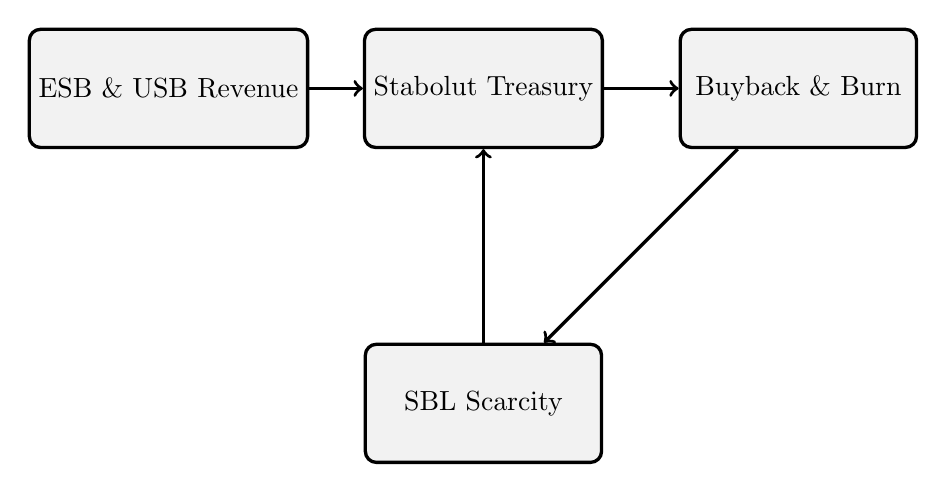
\begin{tikzpicture}
    [
        node/.style={rectangle, rounded corners, draw=black, fill=gray!10, very thick, minimum height=15mm, minimum width=30mm, text centered},
        arrow/.style={->, very thick}
    ]
    % Nodes
    \node[node] (revenue) at (0,0) {ESB \& USB Revenue};
    \node[node] (treasury) at (4,0) {Stabolut Treasury};
    \node[node] (buyback) at (8,0) {Buyback \& Burn};
    \node[node] (scarcity) at (4,-4) {SBL Scarcity};

    % Arrows
    \draw[arrow] (revenue) -- (treasury);
    \draw[arrow] (treasury) -- (buyback);
    \draw[arrow] (buyback) -- (scarcity);
    \draw[arrow] (scarcity) -- (treasury);
\end{tikzpicture}
\caption{The SBL Value-Creation Flywheel}
\label{fig:flywheel}
\end{figure}

\paragraph{The Buyback and Burn Mechanism}
The buyback and burn program is the primary driver of SBL value appreciation. When the Stabolut Treasury's reserves exceed 25\% of the total circulating stablecoin supply (ESB and USB), SBL holders can vote to allocate a portion of the surplus to the buyback and burn mechanism.

The amount to be used for the buyback, $B$, is calculated as follows:
\begin{equation}
B = (\text{Treasury Assets} - (0.25 \times \text{Circulating Stablecoin Supply})) \times \text{Burn Allocation \%}
\end{equation}


The number of SBL tokens to be burned, $SBL_{burned}$, is then determined by the current market price of SBL, $P_{SBL}$:
\begin{equation}
SBL_{burned} = \frac{B}{P_{SBL}}
\end{equation}

This process has a direct and immediate impact on the circulating supply of SBL, which in turn affects its market price. The new theoretical price of SBL, $P_{SBL'}$, can be modeled as:
\begin{equation}
P_{SBL'} = \frac{\text{SBL Market Cap}}{\text{Circulating Supply} - SBL_{burned}}
\end{equation}

This deflationary pressure, combined with the ongoing revenue generation from the ESB and USB ecosystems, creates a powerful and sustainable value accrual model for SBL holders.

The total value of the SBL token can be conceptualized as the sum of its base utility value, the net present value (NPV) of its future revenue share, the NPV of its future treasury surplus distributions, and a scarcity premium derived from the buyback and burn program.

\begin{equation}
\text{SBL Value} = \text{Base Utility} + \text{NPV(Revenue Share)} + \text{NPV(Surplus Distributions)} + \text{Scarcity Premium}
\end{equation}


\subsection{Regulatory Compliance and Investor Protection}

The SBL value accrual framework is designed to be fully compliant with the Markets in Crypto-Assets (MiCA) regulation. By structuring SBL as a utility token with governance rights and making distributions non-guaranteed and community-controlled, Stabolut mitigates the risk of SBL being classified as a security.

Key compliance features include:
\begin{itemize}
    \item \textbf{MiCA-Compliant Framework}: The SBL tokenomics are designed to align with MiCA's requirements for utility tokens.
    \item \textbf{Governance Control}: SBL holders have full control over the treasury surplus distribution, ensuring a decentralized and democratic process.
    \item \textbf{Legal Oversight}: All major governance decisions are subject to legal review to ensure ongoing compliance with MiCA and other global regulations.
\end{itemize}

